%\VignetteIndexEntry{ImageMetrics Analysis of images for social scientists}
\documentclass[12pt]{article}
%\usepackage[OT1]{fontenc}
%\usepackage{babel}
%\usepackage{hyperref} 
\usepackage{url}   %this allows us to cite URLs in the text
\usepackage{graphicx}  %allows for graphic to float when doing jou or doc style
\usepackage{amssymb}  %use formatting tools  for math symbols
\usepackage{natbib}  %might conflict with apa...
\usepackage{booktabs}
\usepackage{fullpage}
\usepackage{setspace} 
% Sweave & pgfSweave
\usepackage{Sweave}
%\usepackage{tikz}
%\usepackage{pgf}
\begin{document}  
\title{R package vignette for ImageMetrics:\\ Analysis of images for social scientists}
\author{Solomon Messing}

\maketitle

\def\Sweavesize{\smallsize}
\DefineVerbatimEnvironment{Sinput}{Verbatim} {xleftmargin=1em}
\DefineVerbatimEnvironment{Soutput}{Verbatim}{xleftmargin=1em}
\DefineVerbatimEnvironment{Scode}{Verbatim}{xleftmargin=1em}



\tableofcontents

\section{Introduction}

In life and in politics, images matter.  The nation's first televised debate on September 26, 1960 fundamentally re-defined what it meant to be a political success in America---you needed to look presidential.  It is now widely recognized that those who watched the debates on television saw a pale and underweight Nixon losing the debate to a calm and confident Kennedy, while the few who listened in via radio thought Nixon won.  Images are just as important today: witness remarks by Harry Ried during the early stages of the Obama primary campaign, suggesting he was ``impressed'' by Obama's light skin and lack of dialect.  Shortly after, the Political Communication Lab at Stanford conducted a series of experimental studies, which found that viewing political advertisements with darker images of Obama had a negative impact on respondents' preference for Obama as a presidential candidate during the early stages of the campaign \citep{iyengar2010explicit}.     

The \texttt{ImageMetrics} package provides researchers with a number of useful tools for the study of images in social science.  It allows researchers to import image data from .jpg and .png files (using the \texttt{png} and \texttt{ReadImages} packages), and to generate RBG and HSV readings for hand-selected portions of an image, which is useful when analyzing particular objects in an image such as a face.  Though many GUI based image processing software packages such as Photoshop allow users to get RGB and HSV metrics from a small range of pixels, this is the first package of which I am aware that allows the user to get these metrics from an object that is selected within an image.  Furthermore, the fact that the package exists within the R environment means that saving the results of processing many different images is less suseptible to errors related to transcription.  

Perhaps most useful for social scientists is the capability to generate HSV (Hue, Saturation, and Value (brightness)) metrics to describe each image or a particular portion of an image, which correspond respectively to the color, color intensity, and the lightness/darkness of an image.  For example, in \citet{messing2009Bias}, a similar approach was used to document that the 2008 McCain campaign used more images that portrayed Obama's skin complexion significantly darker in attack ads, and that both campaigns used images of their opponents with markedly low color saturation in attack advertisements.  This vignette will document the process by which one goes about hand-selecting objects in images for analysis (e.g., faces) and how this package can be used to generate meaningful metrics with respect to the results. 

\section{Reading in Images}
Reading in images is best done via the \texttt{readPNG()} function, part of package \texttt{png}.  This function will read in a PNG file and return a three- or four-dimensional array representing each pixel of the original image, in red-blue-green (RGB) or red-blue-green-alpha (RGBA) format.  The first two dimensions are the x and y coordinates of the image, while the third dimension represents each color ``slice'' of an image.       

\begin{Schunk}
\begin{Sinput}
 options(prompt = " ", continue = " ", width=40)
 library(ImageMetrics)
 image = new("imageMatrix", 
 		X = readPNG(system.file("extdata", "jm-sep25-promise1.png", 
 						package="ImageMetrics")), 
 		type = "rgba")
 str(image)
\end{Sinput}
\begin{Soutput}
Formal class 'imageMatrix' [package "ImageMetrics"] with 6 slots
  ..@ .Data : num(0) 
  ..@ X     : num [1:578, 1:623, 1:3] 0 0 0 0 0 0 0 0 0 0 ...
  ..@ type  : chr "rgba"
  ..@ imgdim: num [1:3] 578 623 3
  ..@ ncol  : int 578
  ..@ nrow  : int 623
\end{Soutput}
\end{Schunk}

Users can access the actual pixel-by-pixel image data via \texttt{image@X}.  

It is also possible to read in images using the \texttt{read.jpeg()} function, though it fails to read in some jpeg images.    

If the image corpus in question is in a different format, it is relatively easy to use the powerful cross-platform application \texttt{ImageMagick} to convert a large batch of images from one type to another, available at \url{http://www.imagemagick.org/script/index.php}.     

\section{Hand-selecting objects in images}
The \texttt{ImageMetrics} package provides a primitive but effective \texttt{tcltk} interface to allow users to selection a portion of an image for further analysis.  In order to hand-select an object within an image, we need to represent the object as a polygon, with points corresponding to pixel locations in the original image.  This can be done using the \texttt{setObjPoly} and \texttt{getObjPoly} functions.  The former brings up a \texttt{tcltk} interface wherein the user clicks on various points to outline an object in the image.  In the current implementation, no markers appear on screen telling the user where he or she has just clicked.  Nonetheless, the system does record those pixels.  The latter, \texttt{getObjPoly}, retrieves the points where the user selected, and converts them to approximate image coordinates.  Here, C code from the \texttt{maps} package is utilized to quickly determine which points are within the polygon.


\setkeys{Gin}{width=0.45\textwidth}
\begin{figure}[ht]
\centering
\caption{An image and object selected from it}
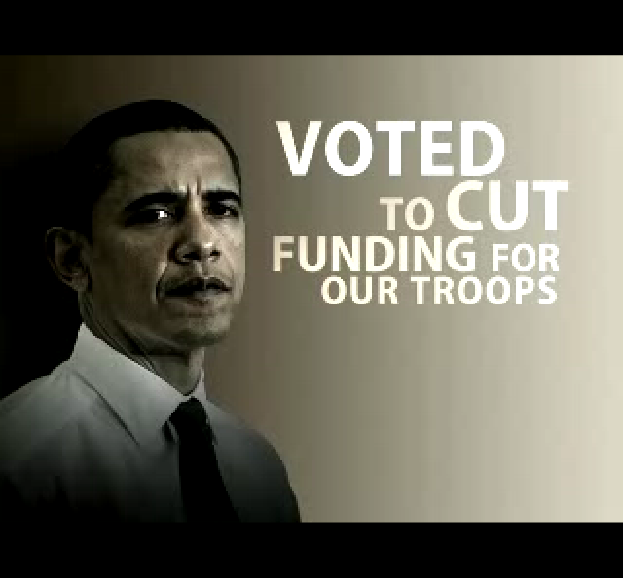
\includegraphics{jm-sep25-promise1.png}
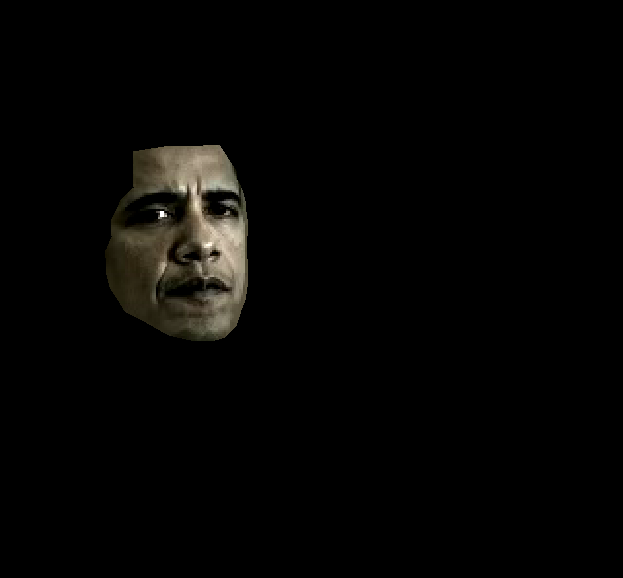
\includegraphics{obamaface.png}
\label{fig:jmfamily}
\end{figure}


When processing a large batch of images, users may find it more beneficial to go about creating these polygons in a corpus of images by utilizing the interface provided with Bio7, a Windows and Linux development environment originally designed for ecological modeling, available at \url{http://sourceforge.net/projects/bio7/}.  Bio7 provides an excellent interface with which one can outline a polygon in an image and send the image's coordinates to R.  With a little bit of scripting, a system can be set up to easily extract the coordinates from an image.  For useful scripts and/or advice on setting up a system, please contact the package author \texttt{[lastname] at stanford dot edu}.  This was the system used to gather polygons in \citet{messing2009Bias}.      

\begin{figure}[ht]
\centering
\caption{Using Bio7 to capture polygon coordinates corresponding to an object}
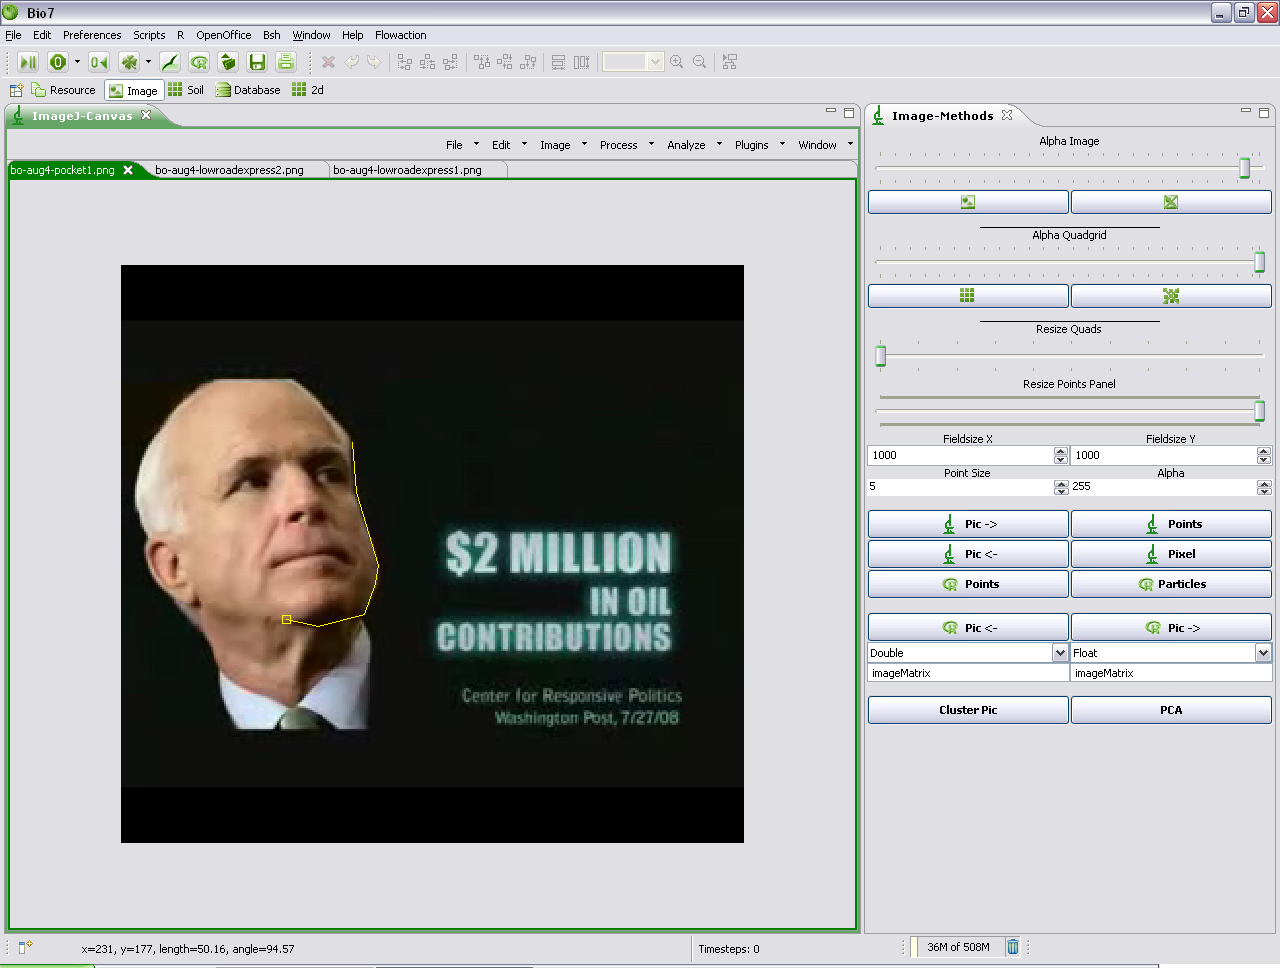
\includegraphics{CodingMcCain.png}
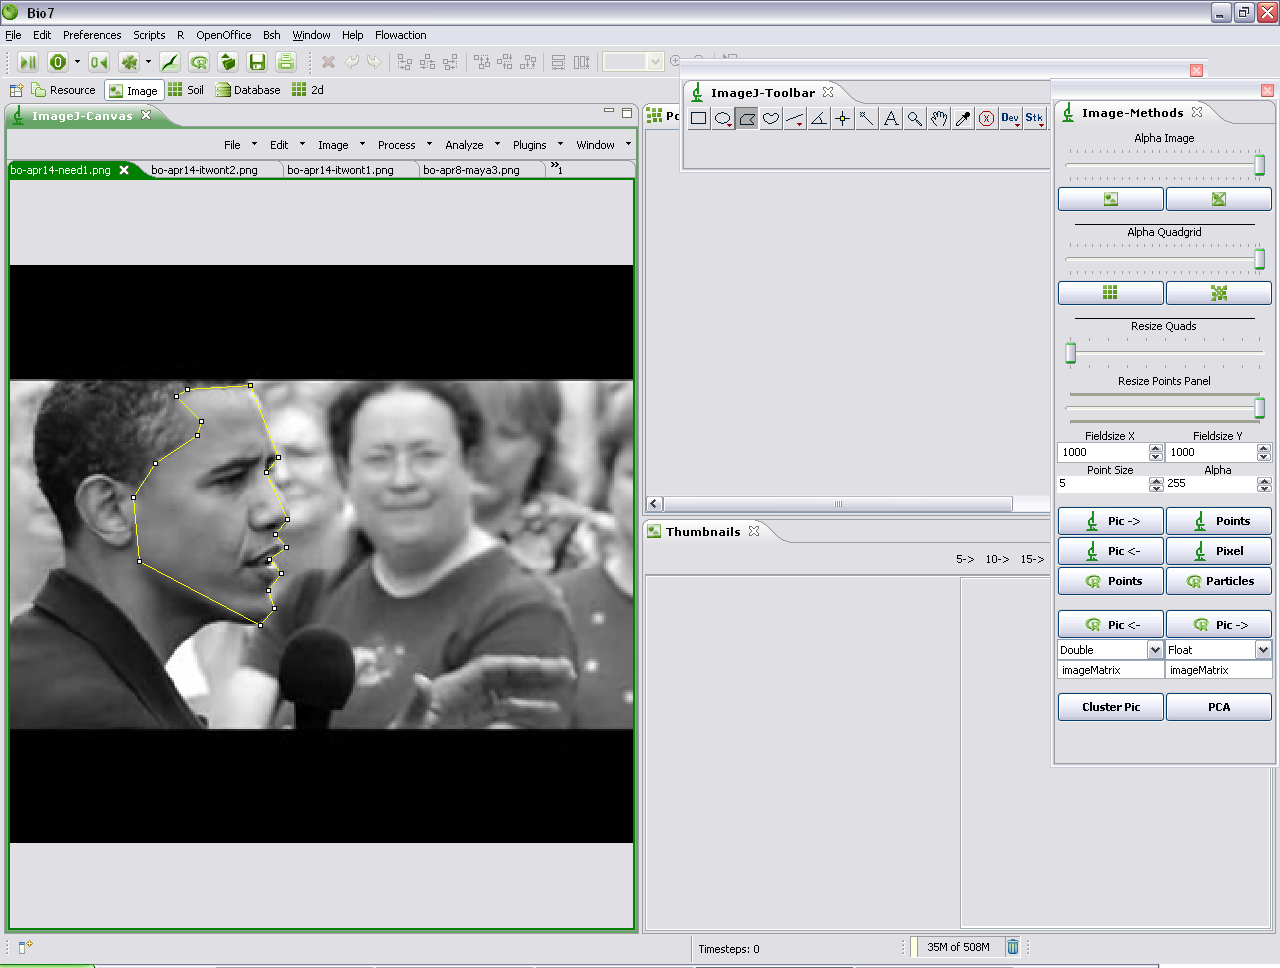
\includegraphics{Instructions2.png}
\label{fig:jmfamily}
\end{figure}

Future implementations will attempt to incorporate bindings for the \texttt{OpenCV} package for C++, which has facilities to automatically detect faces and other objects in images.  When this capability is implemented, the \texttt{tcltk} interface will serve as a useful tool to develop training data sets for more complicated image and video processing tasks such as face delineation (post-detection) and expression classification.  

\section{Creating new images from selection}
Next, users should use the \texttt{ObjSelect} function, which uses C code from the \texttt{maps} package to detect which pixels in the image are within the polygon that the user selected, and put the results in an imageMatrix.  This function sets all pixels that are not located in the package to NA.  Then, appropriate metrics can be extracted from the image or image selection.  When the plot function is called on an S4 \texttt{imageMatrix} object, these NA pixels show up as black in the image.  Writing the output to a file can currently only be accomplished by calling the \texttt{writePNG} function from the \texttt{png} package.

\begin{Schunk}
\begin{Sinput}
 mcattackad = new("imageMatrix", 
 	X = readPNG(system.file("extdata", "jm-sep25-promise1.png", 
 			package="ImageMetrics")), 
 	type = "rgba")
 ## opens tcltk interface
 setObjPoly(mcattackad) 
 ## returns polygon corresponding to the object the user selected.
 mcattackadpoly = getObjPoly(mcattackad) 
 # create new image with only the object selected.
 mcattackadface = new("imageMatrix", 
 	X = ObjSelect( image = mcattackad@X, poly= mcattackadpoly ), 
 	type = "rgb")
 plot(mcattackadface)
 writePNG(mcattackadface@X, "obamaface.png")
\end{Sinput}
\end{Schunk}

\section{Generating metrics and density plots}
The \texttt{ImageMetrics} package provides red-blue-green (RGB) and hue-saturation-value (HSV) metrics for an image or image selection.  In the example below, we compare the brightness of a video still capture from MSNBC footage of Obama, with a still capture from an ad featuring the same footage that appeared in an ad on the Clinton campaign website.  Obama appeared significantly darker and stretched horizontally in the Clinton ad, which exaggerated Obama's Afrocentric facial features.  This caused quite a stir among Democrat bloggers, most notably ``Troutnut,'' who accused the Clinton campaign of using racial bias as tool in attack advertising \citep{troutnut2008hillarys}.  Though the distortion may be a product of video software and/or compression, the racial sensitivities surrounding Obama's primary candidacy, along with the campaign's subsequent denial that they produced the ad \citep{fox2008questions} made the Clinton campaign appear clumsy at best.  

\setkeys{Gin}{width=0.45\textwidth}
\begin{figure}[ht]
\centering
\caption{Video still capture from original MSNBC footage (via YouTube) and ad on Clinton campaign website}
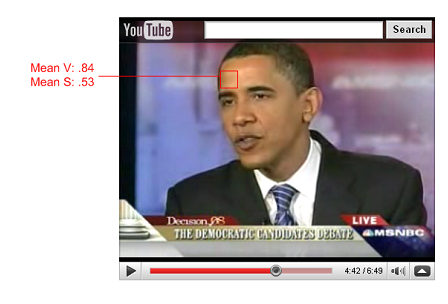
\includegraphics{MSNBC.png}
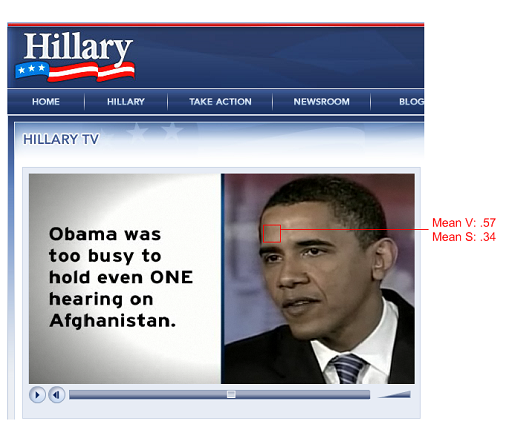
\includegraphics{Clinton.png}
\label{fig:clintad}
\end{figure}

The images in Figure~\ref{fig:clintad} above show video stills that I captured from the Clinton campaign website and the original MSNBC footage (from YouTube).  The package includes the polygons that correspond to the facial coordinates of Obama's face in each image \texttt{clintonpoly} and \texttt{msnbcpoly} respectively, so we simply create a new image from those coordinates, make sure the polygon is capturing the correct portion of the image via the \texttt{plot} function, and generate saturation and value readings.       

\begin{Schunk}
\begin{Sinput}
 data(Campaign2008)
 clinton = new("imageMatrix", 
 	X = readPNG(system.file("extdata", "Clinton.png", package="ImageMetrics")), 
 	type = "rgba")
 clintonface = new("imageMatrix", 
 	X = ObjSelect( image = clinton@X, poly= clintonpoly ), 
 	type = "rgb")
 plot(clintonface)
 msnbc = new("imageMatrix", 
 	X = readPNG(system.file("extdata", "MSNBC.png", package="ImageMetrics")), 
 	type = "rgba")
 msnbcface = new("imageMatrix", 
 	X = ObjSelect( image = msnbc@X, poly= msnbcpoly ), 
 	type = "rgb")
 plot(msnbcface)
 clinthsv = meanhsv(clintonface)
 msnbchsv = meanhsv(msnbcface)
 msnbchsv$V
\end{Sinput}
\begin{Soutput}
[1] 0.6604202
\end{Soutput}
\begin{Sinput}
 clinthsv$V
\end{Sinput}
\begin{Soutput}
[1] 0.4671259
\end{Soutput}
\begin{Sinput}
 # Clinton ad darker
 
 msnbchsv$S
\end{Sinput}
\begin{Soutput}
[1] 0.5166407
\end{Soutput}
\begin{Sinput}
 clinthsv$S
\end{Sinput}
\begin{Soutput}
[1] 0.3666436
\end{Soutput}
\begin{Sinput}
 # and less saturated with color
\end{Sinput}
\end{Schunk}

We would also like the capability for storing image coordinates for later batch processing.  We can create a data frame or list object with the image names and polygon coordinates.  

\begin{Schunk}
\begin{Sinput}
 data(Campaign2008)
 # Replace the following line with any system directory containing images 
 imagedir = system.file("extdata", package="ImageMetrics")
 imagedir
 # NOTE: files cannot have "-" characters in them!
 for(i in 1:length(filenames)){
 	file.rename(from = paste( imagedir, "/", filenames[i], sep=""), 
 	to = paste( imagedir, "/", 
 	gsub( pattern = "\\-", replacement = "", filenames[i]), sep=""))
 }
 # update filenames in directory 
 filenames = dir(imagedir)
 filenames
 # create an imageMatrix object for every file in the directory
 for(img in filenames){
 	eval(parse(text=paste(img, 
 	" = new(\"imageMatrix\", 
 	  X =  readPNG(paste( imagedir, \"/\", img, sep=\"\")), type = \"rgba\")"
 		) ))
 }
 # Hand-select the polygon for each image:
 i = 1
 # opens tcltk interface
 setObjPoly( eval(parse(text=filenames[i])) ) 
 # returns polygon corresponding to the object the user selected.
 eval( parse( text = paste(filenames[i], 
 		"poly = getObjPoly(eval(parse(text=filenames[i])))", 
 		sep=".")))  
 # Repeat, increasing the index i for each photo...
 
 # When done with every file, create data object:
 objectlist = list()
 for(i in 1:length(filenames)){
 	# store polygon in list
 	eval(parse(text=paste("objectlist$", 
 		filenames[i], "$poly=", filenames[i], ".poly", sep=""))) 
 	
 	# store hsv in list:
 	eval(parse(text=paste("objectlist$", filenames[i], 
 		"= meanhsv( new(\"imageMatrix\", X = ObjSelect( image = ", 
 		filenames[i], 
 		"@X, poly=", filenames[i], ".poly ), type = \"rgb\"))",
 		sep="") ))
 }
 
\end{Sinput}
\end{Schunk}

It is also sometimes desirable to produce a density plot showing the distribution of pixels.  Functions \texttt{svhist}, \texttt{huehist}, and \texttt{rgbhist} are built in to the \texttt{ImageMetrics} package produce plots showing the density of saturation and value, hue, and red-, green-, and blue- channel intensity in the imageMatrix object.    

\setkeys{Gin}{width=0.9\textwidth}
\begin{figure}[ht]
\caption{Histograms describing saturation and value of Clinton and MSNBC images}
\begin{Schunk}
\begin{Sinput}
 par(mfrow = c(1,2), cex = .7)
 svhist(msnbcface, main = "MSNBC")
 svhist(clintonface, main = "Clinton" )
\end{Sinput}
\end{Schunk}
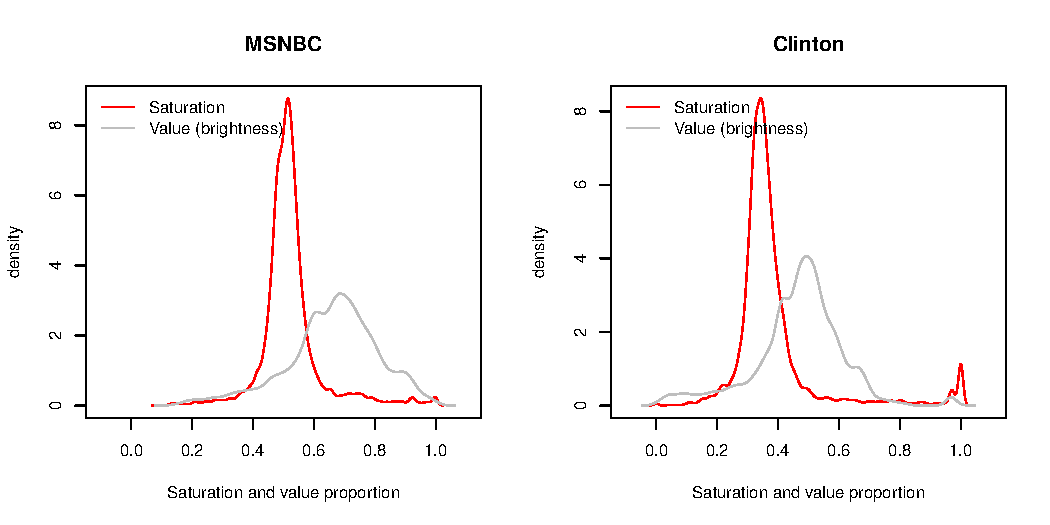
\includegraphics{ImageMetrics-svhist}
\label{fig:clmsn}
\end{figure}

Based on the density plots of Obama's face in each ad, we can see that the Clinton ad is much darker and has significantly lower color saturation than does the original footage.  Furthermore, the image in the ad appears to have higher contrast, with tighter spikes at about .35 and 1 than in the original MSNBC footage.      

\newpage

\bibliographystyle{apalike}
\bibliography{Race}  

\end{document}
